% !TEX root =./main.tex

\section{Block 7: Scan Conversion - Cometto}

Scan conversion handles the task of converting the stored beam data (in our case, in Mag\_image) from its polar reference (beam/sample or angle/distance) to a rectangular reference that can be used as data for an image.  Additionally, in order to form a continuous image, the values between the beams must be interpolated.

\subsection{Background}

Before discussing the implementation, we will first discuss the information necessary to understand and accomplish this task.  First, the signal data is stored in an array named \code{Mag\_image} where each row corresponds to a beam (angle), and each column corresponds to a sample (distance).  In our case, the array is $21 \times 4000$.  The output of the scan conversion stage is a $100 \times 201$ pixel image, which will be stored as a $100 \times 201$ array called \code{image}.

We will define the pixel at index $(1,101)$ as our position $(x,y) = (0,0)$.  From there, we can assign each pixel an angle, $\theta_p$, and a distance, $r_p$.  Then, we can perform bilinear interpolation using the equation
\begin{align*}
    \code{image[r,c]} = (1-\beta) &\left( (1 - \alpha) \code{Mag\_image[k,n]} + (\alpha) \code{Mag\_image[k+1,n]}  \right) \\ 
    + (\beta) &\left( (1-\alpha) \code{Mag\_image[k,n+1]} + (\alpha) \code{Mag\_image[k+1,n+1]} \right)
\end{align*}
with
\begin{align*}
    \alpha = \frac{\theta_p - \theta_n}{\theta_{n+1} - \theta_n}
\end{align*}
and
\begin{align*}
    \beta = \frac{r_p - r_n}{r_{n+1} - r_n}
\end{align*}
as the fractional offsets in the angle and distance directions, respectively.  This allows us to use use a weighted average of the four nearest known values to calculate the value at every pixel of the output image.

\subsection{Implementation}

In order to implement this algorithm in a fast way, we need to precompute as much as possible.  With the right values precomputed, it is possible to completely vectorize the function, as is done in \code{scan\_conversion.m}.  Ultimately, we need $8$ precomputed values, described in Table \ref{tab:precomputeScan}.

\begin{table}[H]
    \centering
    \begin{tabular}{cc}
        Parameter & Description  \\ \hline
        \code{ind\_bkn} & Set of linear indices for the $(k,n)$ value for each pixel \\
        \code{ind\_bk1n} & Set of linear indices for the $(k+1,n)$ value for each pixel \\
        \code{ind\_bkn1} & Set of linear indices for the $(n,k+1)$ value for each pixel \\
        \code{ind\_bk1n1} & Set of linear indices for the $(n+1,k+1)$ value for each pixel \\
        \code{BMAM} & The value of $(1-\beta)(1-\alpha)$ for each pixel \\
        \code{BMA} & The value of $(1-\beta)(\alpha)$ for each pixel \\
        \code{BAM} & The value of $(\beta)(1-\alpha)$ for each pixel \\
        \code{BA} & The value of $(\beta)(\alpha)$ for each pixel \\
    \end{tabular}
    \caption{Precomputed Values for Scan Conversion}
    \label{tab:precomputeScan}
\end{table}

In addition, we are able to calculate the feet per pixel in both the $x$-direction and $y$-direction.  This reveals that a $100 \times 201$ pixel image has a ratio of $\frac{y_{feet}}{x_{feet}}$ that is very close to one, which enables easy interpretation of the output image.

To do these precalculations, we first need the distance and angle of each pixel.  We first find the rectangular coordinates $(p_x, p_y)$ of the pixel at index $[p_r,p_c]$ with
\begin{align*}
    p_y = \frac{\code{image\_rows} - 1}{r_{max}}
\end{align*}

\begin{align*}
    p_x = 
\end{align*}


find them with
\begin{align*}
    r_p = \sqrt{(s_yp_r)^2 + (s_xp_c)}
\end{align*}


In order to find the $k$ and $n$ indices corresponding to each image pixel, we calculate 
\begin{align*}
    k_p = \frac{F_s\sin(\theta_p)}{2 f_c}
\end{align*}
and
\begin{align*}
    n_p = \frac{cr_p}{F_s}
\end{align*}
for speed $c$, frequency of the pulse $f_c$, and sampling frequency $F_s$.





















We must implement both of these steps in a very fast way, without sacrificing quality.

First, \textsc{Matlab} is meant for working with vectorized functions, and has vectorized methods of replacing certain indexes.  Thus, the quickest way to add a zero after every sample (double the number of samples) is to replace every other entry of a matrix of zeros with the data point.

Second, in order to interpolate, we will use the minimum order filter possible that preserves the necessary information, because a lower order results in less multiplies and thus a quicker function.  Additionally, FIR was chosen in order to preserve the relative phase of the received signals, which is necessary for preventing distortion in the sonar image.  Equirriple was used as the design method.

In this case, an order 3 filter with the specifications in Table \ref{tab:upsample_filter} works.  Our information is contained in the band less than $20 \unit{kHz}$, and thus we can set $f_{pass}$ to $20 \unit{kHz}$.  Then, because our $F_{s,old} = 100 \unit{kHz}$, there is a significant amount of bandwidth between our data's frequency spectrum and its reflected image.  Thus, we can set $f_{stop}$ to be $69 \unit{kHz}$, the sharpest it can be while still being order 3.  Through various trials, an $A_{stop}$ of $40 \unit{dB}$ sufficiently suppresses the image, will also allowing the filter to be order 3.

\begin{table}[H]
    \centering
    \begin{tabular}{c|cccc}
        Order & Fpass & Fstop & Apass & Astop \\ \hline
        3 & $20  \unit{kHz}$ & $69  \unit{kHz}$ & $1  \unit{dB} $ & $40  \unit{dB}$
    \end{tabular}
    \caption{Parameters for Upsampling Low Pass Filter}
    \label{tab:upsample_filter}
\end{table}

The frequency response of the low pass filter can be seen in Figure \ref{fig:upsample_freq_response}.

\begin{figure}[H]
    \centering
    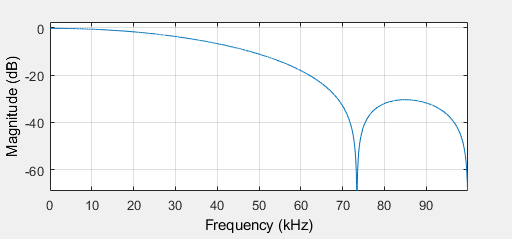
\includegraphics[width=0.5\linewidth]{figures/upsample_freq_response.png}
    \caption{Frequency Response of Upsampling Low Pass Filter}
    \label{fig:upsample_freq_response}
\end{figure}

In order to preserve this speed, the function header was modified to accept the numerator taps of the low pass filter, matrix of zeros, and the length of the matrix of zeros as input in addition to the data to be upsampled.


\subsection{Analysis}

An initial, simple test to confirm that the function upsamples properly is by inspecting a linear function.  This can be seen in Figure \ref{fig:linear_upsample_whole}. 

\begin{figure}[H]
    \centering
    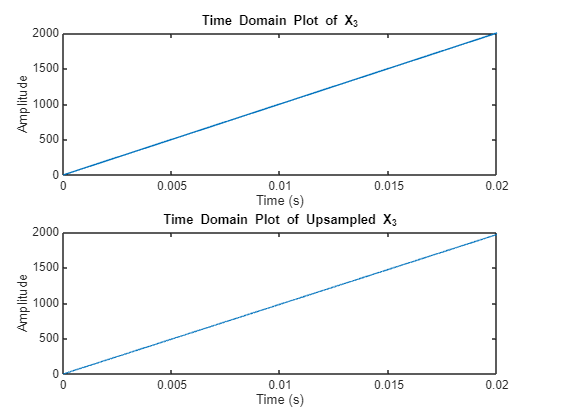
\includegraphics[width=0.5\linewidth]{figures/linear_upsample_whole.png}
    \caption{Upsampled Linear Function}
    \label{fig:linear_upsample_whole}
\end{figure}

It can be seen  in Figure \ref{fig:linear_upsample_zoom} that the upsampled version contains the same data, but has twice as many points.

\begin{figure}[H]
    \centering
    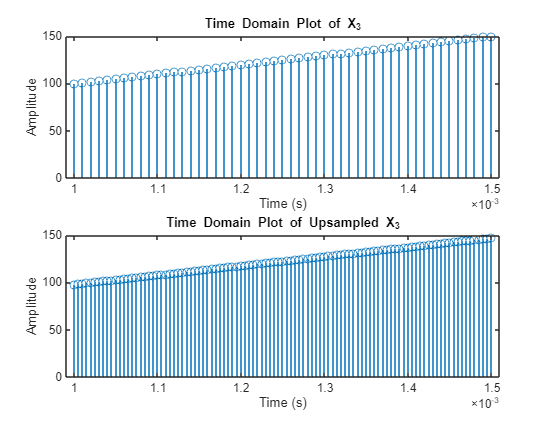
\includegraphics[width=0.5\linewidth]{figures/linear_upsample_zoom.png}
    \caption{Zoomed Portion of Upsampled Linear Function}
    \label{fig:linear_upsample_zoom}
\end{figure}

Testing on various other types of synthetic data, such as sinusoids and linear combinations of sinusoids, further confirmed that the function was implemented as intended.  

As the next test, we can upsample the provided test data (unmodified by the other stages) to ensure it has no unintended effects.  As can be seen in Figure \ref{fig:upsample_time} and Figure \ref{fig:upsample_freq}, the data was interoplated correctly.  Each channel is represented by a color.

\begin{figure}[H]
    \centering
    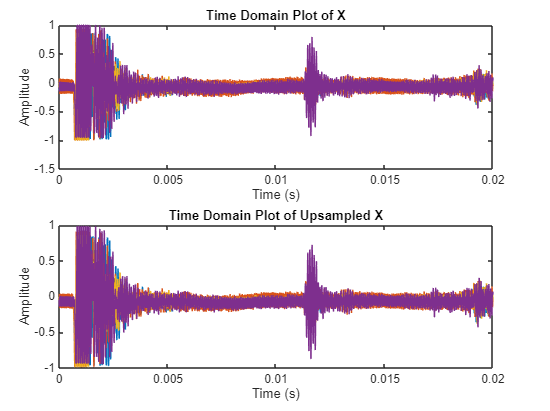
\includegraphics[width=0.5\linewidth]{figures/upsample_time.png}
    \caption{Upsampled Data in Time}
    \label{fig:upsample_time}
\end{figure}

\begin{figure}[H]
    \centering
    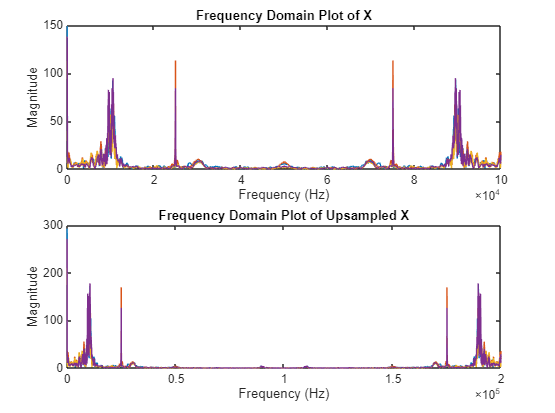
\includegraphics[width=0.5\linewidth]{figures/upsample_freq.png}
    \caption{Upsampled Data in Frequency}
    \label{fig:upsample_freq}
\end{figure}

Zooming in for Figure \ref{fig:upsample_time_zoom} and Figure \ref{fig:upsample_freq_zoom}, we can more clearly see that the interpolation was successful.

\begin{figure}[H]
    \centering
    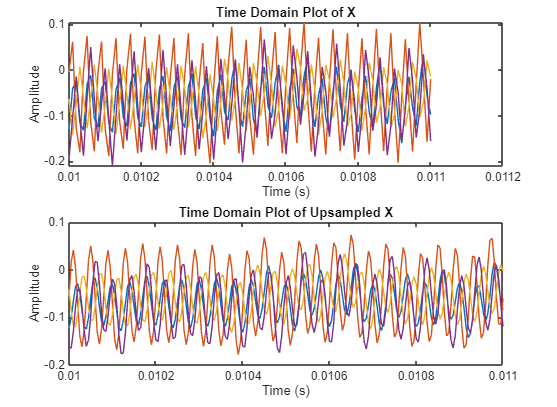
\includegraphics[width=0.5\linewidth]{figures/upsample_time_zoom.png}
    \caption{Zoomed Portion of Upsampled Data in Time}
    \label{fig:upsample_time_zoom}
\end{figure}

\begin{figure}[H]
    \centering
    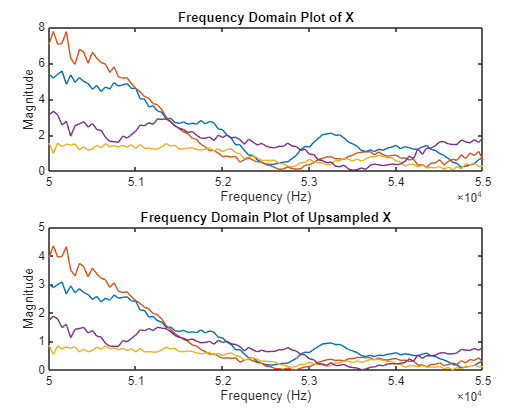
\includegraphics[width=0.5\linewidth]{figures/upsample_freq_zoom.png}
    \caption{Zoomed Portion of Upsampled Data in Frequency}
    \label{fig:upsample_freq_zoom}
\end{figure}

Therefore, the function successfully interpolates the data at a high quality.  The next step in the analysis is in the timing.  Benchmarking is difficult, but here we are only comparing the newly written function to the provided \code{.p} file.  In this case, each function was timed (using \code{tic} and \code{toc}) over $10,000$ iterations, and the average runtimes can be seen in Table \ref{tab:upsampleFunctionTime}.  The same data (the provided test data) was used, and the computer was in as similar a state as possible.

\begin{table}[H]
    \centering
    \begin{tabular}{cc}
        Function & Time ($\mu$s) \\ \hline
        Provided \code{.p} & $5455$\\
        Rewritten \code{.m} & $64.7$
    \end{tabular}
    \caption{Provided vs Rewritten Upsampling Function Performance}
    \label{tab:upsampleFunctionTime}
\end{table}

Therefore, the rewritten \code{upsampling.m} function provides a high quality upsampling by $2$ and is about 100 times faster than the original function.